\documentclass{standalone}
\usepackage{tikz}
\usepackage{ctex,siunitx}
\usepackage{tkz-euclide}
\usepackage{amsmath}
\usetikzlibrary{patterns, calc}
\usetikzlibrary {decorations.pathmorphing, decorations.pathreplacing, decorations.shapes,}
\begin{document}
\small
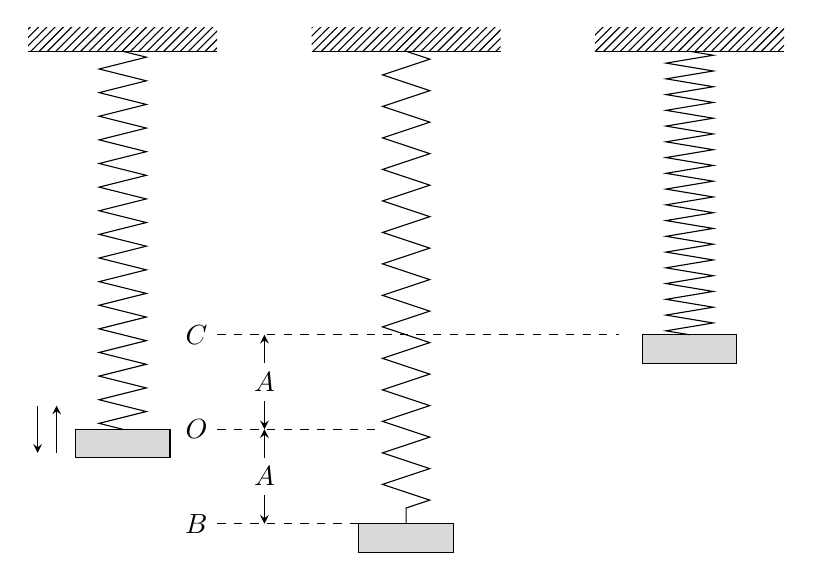
\begin{tikzpicture}[>=stealth,scale=1.2]
  \tikzstyle{spring1}=[decorate,decoration={aspect=0.5, segment length=4mm, amplitude=3mm,zigzag}]
  \tikzstyle{spring2}=[decorate,decoration={aspect=0.5, segment length=3mm, amplitude=3mm,zigzag}]
  \tikzstyle{spring3}=[decorate,decoration={aspect=0.5, segment length=2mm, amplitude=3mm,zigzag}]
  \fill [pattern = north east lines] (-4,0) rectangle (-2,.25);
  \fill [pattern = north east lines] (-1,0) rectangle (1,.25);
  \fill [pattern = north east lines] (2,0) rectangle (4,.25);
  \draw(-4,0)--(-2,0);  \draw(-1,0)--(1,0);  \draw(2,0)--(4,0);
  \draw [fill=gray!30] (-3.5, -4.3) rectangle (-2.5, -4);
  \draw [fill=gray!30] (-.5, -5.3) rectangle (.5, -5);
  \draw [fill=gray!30] (2.5, -3.3) rectangle (3.5, -3);
  \draw [spring2](-3,0)--(-3,-4);
  \draw [spring1](0,0)--(0,-5);
  \draw [spring3](3,0)--(3,-3);
  \draw [dashed](-2, -3)node[left]{$C$}--(2.25,-3);
  \draw [dashed](-2, -4)node[left]{$O$}--(-.25,-4);   
  \draw [dashed](-2, -5)node[left]{$B$}--(-.25,-5);   
  \draw [<->](-1.5, -3)--node[fill=white]{$A$}(-1.5,-4);
  \draw [<->](-1.5, -5)--node[fill=white]{$A$}(-1.5,-4);
  \draw [->] (-3.7, -4.25)--(-3.7, -3.75);
  \draw [<-] (-3.9, -4.25)--(-3.9, -3.75);
\end{tikzpicture}
\end{document}